\documentclass[a4paper]{article}

%maximum figure number
\setcounter{totalnumber}{5}

%plus minus
\newcommand{\mypm}{\mathbin{\smash{%
\raisebox{0.35ex}{%
            $\underset{\raisebox{0.5ex}{$\smash -$}}{\smash+}$%
            }%
        }%
    }%
}


%figure inside text
\usepackage{wrapfig}

%layout config
\usepackage{calc}
\setlength\textwidth{7in}
\setlength\textheight{10in}
\setlength\oddsidemargin{(\paperwidth-\textwidth)/2 - 1in}
\setlength\topmargin{(\paperheight-\textheight
-\headheight-\headsep-\footskip)/2 - 1in}

%sinuit
\usepackage{siunitx}
%image insertion
\usepackage{graphicx} %image settings
\DeclareGraphicsExtensions{.pdf,.png,.jpg}

%math
\usepackage{amsmath} %math
%\usepackage{cmbright} %math font

%font
\usepackage{kotex}
\usepackage{fontspec}
\ifx가가
\setmainhangulfont[Ligatures=TeX,
BoldFont={KoPubBatang Medium}]{KoPubBatang Light}
\setsanshangulfont[Ligatures=TeX,
BoldFont={KoPubDotum Medium}]{KoPubDotum Light}
\setmainhanjafont[Ligatures=TeX,
BoldFont={KoPubBatang Medium}]{KoPubBatang Light}
\setsanshanjafont[Ligatures=TeX,
BoldFont={KoPubDotum Medium}]{KoPubDotum Light}
\xetexkofontregime[puncts=prevfont, colons=prevfont, cjksymbols=hangul]{latin}
\fi

%줄간격
\usepackage{setspace}
%\usepackage{indentfirst}
\setstretch{1.2}
\everydisplay{\setstretch{1.2}}

%subfigure
\usepackage{subfigure}

\pagestyle{plain}
\title{물리 실험보고서 1}
\author{이한빈, 의예과 2016-13347}

\begin{document}


\numberwithin{equation}{section}
\maketitle

\section{Introduction}
	전하가 자기장 속에서 운동하면 힘을 받는데 그것을 전자기력이라고 하며 다음과 같이 주어진다.
	\begin{equation}
		\vec{F} = q\vec{v} \times \vec{B}
	\end{equation}
	따라서 만약 전하의 운동방향과 자기장이 수직하면 전하가 받는 힘의 크기는 $F=qvB$이고 방향은 오른손법칙에 의해 결정됨을 알 수 있다.

	이 식으로부터 전류가 자기장에 수직한 방향으로 흐르는 도선이 받는 힘을 계산할 수 있는데 $I=Aevn$과 위 식을 연립하면 다음을 얻는다.
	\begin{equation}
		F = BIL
		\label{eq:current}
	\end{equation}
	따라서 자기장을 구할 수만 있으면 전하나 도선이 그 속에서 받는 힘을 알아낼 수 있다.
	
	\begin{figure}[h]
		\centering
		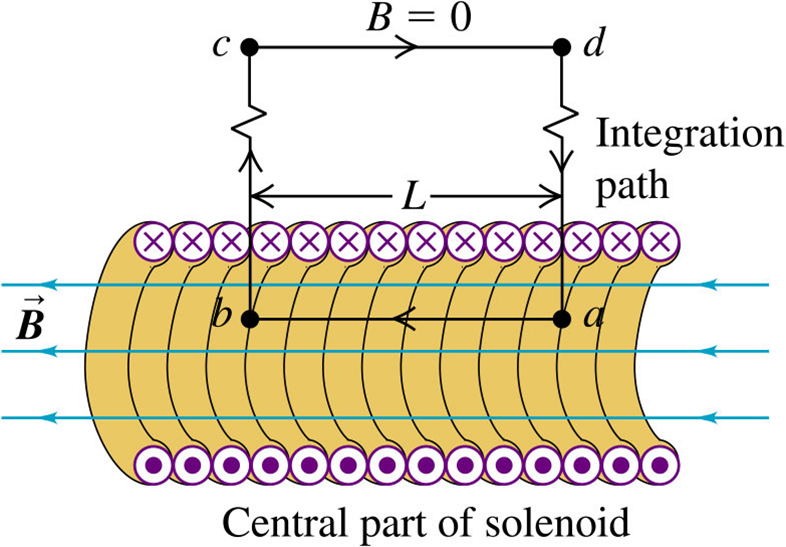
\includegraphics[width=0.4\textwidth]{img/solenoid.png}
		\label{fig:solenoid}
		\caption{솔레노이드와 솔레노이드에 흐르는 전류에 따른 자기장의 방향}
	\end{figure}
	자기장을 발생시키는 장치 중 대표적인 것이 솔레노이드인데 솔레노이드는 원기둥형태로 전선을 일정한 간격으로 감은 장치다.
	솔레노이드의 자기장의 크기는 앙페르 법칙으로 알 수 있으며 그 방향은 그림(\ref{fig:solenoid})처럼 전류방향을 따라 오른손으로 감았을 때 엄지손가락이 가리키는 방향과 같다.

	앙페르 법칙은 흐르는 전류가 만들어내는 자기장을 구할 때 쓰는 식으로 다음과 같이 주어진다.
	\begin{equation}
		\oint \vec{B} \cdot d\vec{s} = \mu{}_{0}I
	\end{equation}

	앙페르 법칙을 이용하여 솔레노이드 내부의 자기장을 구하기 위해 앙페르 폐곡선을 그림(\ref{fig:solenoid})처럼 설정하자.
	폐곡선의 가로길이를 L, 폐곡선을 통과한 전선의 갯수를 N, 솔레노이드 내부의 자기장을 B라고 두면 경로 bc, da의 적분값은 $d\vec{s}$와 $\vec{B}$가 상쇄되어 0이 되고 경로 cd의 적분값은 $B=0$이기 때문에 0이 된다.
	따라서 경로 ab의 적분값만 남게 되어 다음을 얻는다.
	\begin{equation}
		BL = \mu{}_{0}NI
		\label{eq:prosol}
	\end{equation}

	솔레노이드 전선의 간격은 일정하므로 $N/L$은 단위 길이당 감은 전선의 갯수 n과 같음을 알 수 있고 따라서 식(\ref{eq:prosol})의 양변을 L로 나누면 다음을 얻는다.
	\begin{equation}
		B = \mu{}_{0}nI
		\label{eq:sol}
	\end{equation}

	본 실험에서는 일정한 전류가 흐르는 솔레노이드 안에 전류천칭의 도선을 넣고, 전류천칭과 솔레노이드에 흐르는 전류를 바꾸어가며 전류천칭이 기울어지는 정도를 측정했다.
	전류 천칭은 지랫대의 한 쪽 끝에 회전축과 나란한 방향의 전류가 흐르며 무게중심이 받침점 밑에 있는 장치다.
	이를 위해서는 전류천칭에 복원력이 존재해야하는데 전류천칭의 질량중심이 바로 복원력의 원인이다.
	\begin{figure}
		\centering
		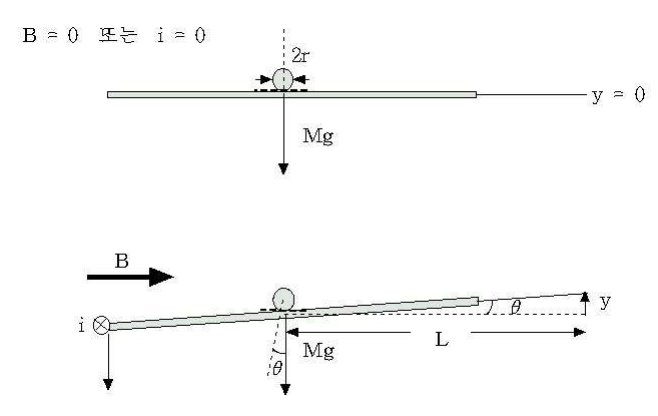
\includegraphics[width=0.5\textwidth]{img/chunching.png}
		\caption{전류천칭과 그 무게중심에 의한 복원력}
		\label{fig:chunching}
	\end{figure}

	그림(\ref{fig:chunching})에서 보여지듯 전류천칭의 무게중심은 받침점 밑에 위치한다.
	따라서 천칭이 각$\theta$만큼 회전하고 나면 천칭의 무게 중심은 받침점을 지나는 수직선을 벗어나 축으로부터 $r\sin{\theta}$만큼의 거리를 갖게 된다.
	받침대의 질량을 $M$라고 하면 이에 의한 회전력은 $Mgr\sin{\theta}$가 된다.
	이때 외력에 의한 토크를 $\tau$이고 $\theta$가 충분히 작으면 다음이 성립한다.
	\begin{equation}
		\tau = Mgr\sin{\theta} = Mgr\theta
	\end{equation}

	그런데 한 쪽 길이 $l$을 알고 있으면 한 쪽 끝이 움직인 거리는 $l\theta$로 주어지므로 천칭의 끝이 움직인 거리를 통해 우리는 토크를 측정할 수 있다.

	이 식을 실제 실험에 맞게 좀 더 정교하게 재구성하자.
	축으로부터 도선의 길이를 a, 받침점 바로 밑에 있는 질량을 $M$, $M$이 매달려 있는 지점과 받침점까지의 거리를 $d$, 그 이외의 질량을 $M'$, 그리고 $M'$가 매달려 있는 위치를 b라고 하자.
	그러면 회전한 각도가 $\theta$로 주어지고 $d$가 $a$나 $b$보다 훨씬 작다고 가정하면 다음과 같은 토크에 대한 평형 방정식을 세울 수 있다.

	\begin{equation}
		F_{전기}a\cos{\theta} + M'gb\cos{\theta} = Mgd\sin{\theta}
		\label{eq:core}
	\end{equation}

	실제 실험에서는 $\theta$의 변화가 매우 작았고 회전축으로부터의 거리가 $l$인 가리키게의 눈금변화 $\Delta{}x$를 측정했기 때문에 식(\ref{eq:core})는 다음과 같이 바꿔 쓸 수 있다. 

	\begin{equation}
		F_{전기} = \frac{1}{a} \cdot (\frac{Mgd\Delta{}x}{l} - M'gb) 
	\end{equation}

	여기서 식(1.2)와 식(1.5)를 결합하면 
	\begin{equation}
		F_{전기} = \mu_{0}ni_{솔}i_{천칭}L
	\end{equation}
	로 주어지므로 $\Delta{}x$가 전류의 변화에 어떻게 반응할 지 예측할 수 있다.

	본 실험에서는 솔레노이드와 전류가 흐르는 도선을 이용하여 토크를 발생시키고, 그 토크를 가리키게의 눈금 변화를 통해 측정함으로써 식(\ref{eq:sol})과 식(\ref{eq:current})을 정량적으로 검증한다.
	
	\newpage

	\section{Method}
	\vspace{-1cm}
		\begin{figure}[h]
			\centering
			\subfigure[오른쪽 직류이중전원장치 왼쪽 전류천칭]{
			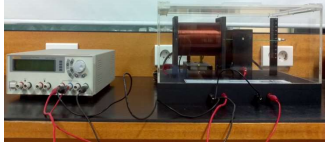
\includegraphics[width=0.4\textwidth]{img/eximg.PNG}
			}
			\subfigure[전류천칭의 회로도]{
			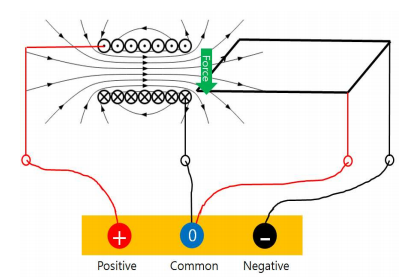
\includegraphics[width=0.4\textwidth]{img/circuit.png}
			\label{fig:circuit}
			}
		\end{figure}
		준비물 : 솔레노이드(길이 12\si{cm}, 감은수 550회), 직류이중전원장치, 집게 전선, 전류 천칭, 마이크로미터
		\subsection{전류천칭의 전류에 따른 토크의 변화}

		\begin{wrapfigure}{r}{0.6\textwidth}
			\centering
            \vspace{-0.5 cm}
			\begin{tabular}{cccccccccc} 
				\hline \hline
				전류(A) \vline & 0.0 & 0.3 & 0.5 & 0.75 & 1.0 & 1.25 & 1.5 & 1.75 & 2.0 \\
				\hline \hline
			\end{tabular}  \vspace{-0.2cm} \caption{천칭에 인가된 전류}
			\vspace{-0.5cm}
			\label{tb:cirinput}
		\end{wrapfigure}
		솔레노이드를 회로도(\ref{fig:circuit})와 같이 되도록 연결했다. 
		전원장치의 전류가 0으로 설정된 것을 확인한 후 전원을 켰다.
		전원장치의 전류와 전압값을 조절하여 천칭의 회로부분이 밑으로 기울어지게 설정했다.
		이때 천칭의 무게 추 쪽 끝이 마이크로미터 기준(가리키게)으로 +0.2\si{cm}가 되도록 했다.
		솔레노이드에 흐르는 전류를 1\si{A}로 고정하고 전류천칭에 흐르는 전류를 표(\ref{tb:cirinput})를 따라 바꿔가며 가리키게의 변위를 측정했다.

		\subsection{솔레노이드의 전류에 따른 토크의 변화}

		\begin{wrapfigure}{r}{0.42\textwidth}
			\centering
            \vspace{-0.5 cm}
			\begin{tabular}{ccccccc} 
				\hline \hline
				전류(A) \vline & 0.0 & 0.5 & 1.0 & 1.5 & 2.0 & 2.5 \\
				\hline \hline
			\end{tabular}  \vspace{-0.2cm} \caption{솔레노이드에 인가된 전류}
			\vspace{-0.5cm}
			\label{tb:solinput}
		\end{wrapfigure}
		솔레노이드를 회로도(\ref{fig:circuit})와 같이 되도록 연결했다. 
		전원장치의 전류가 0으로 설정된 것을 확인한 후 전원을 켰다.
		전원장치의 전류와 전압값을 조절하여 천칭의 회로부분이 밑으로 기울어지게 설정했다.
		이때 천칭의 무게 추 쪽 끝이 마이크로미터 기준(가리키게)으로 +0.2\si{cm}가 되도록 했다.
		전류천칭에 흐르는 전류를 0.5\si{A}로 고정하고 솔레노이드에 흐르는 전류를 표(\ref{tb:solinput})를 따라 바꿔가며 가리키게의 변위를 측정했다.
	
	\newpage

	\section{Result}

		\subsection{전류천칭의 전류에 따른 토크의 변화}

		\begin{figure}[h]
			\centering
			\begin{tabular}{cccccccccc} 
				\hline \hline
				전류(\si{A})   \qquad \qquad \vline & 0.0 & 0.3 & 0.5 & 0.75 & 1.0 & 1.25 & 1.5 & 1.75 & 2.0 \\
				\hline
				가리키게 눈금(\si{cm}) \vline & 9.9 & 9.9 & 9.9 & 9.9 & 9.9 & 10 & 10 & 10 & 10 \\
				\hline
				가리키게 변위(\si{cm}) \vline & 0.2 & -0.0 & -0.1 & -0.4 & -0.6 & -0.8 & -1.2 & -1.4 & -1.7 \\
				\hline \hline
			\end{tabular}  
			\label{tb:cirouput}
		\end{figure}

		\vspace{-0.5cm}

		\begin{figure}[h]
			\centering
			\subfigure[천칭에 인가된 전류와 그에 따른 가리키게의 위치 변화]{
				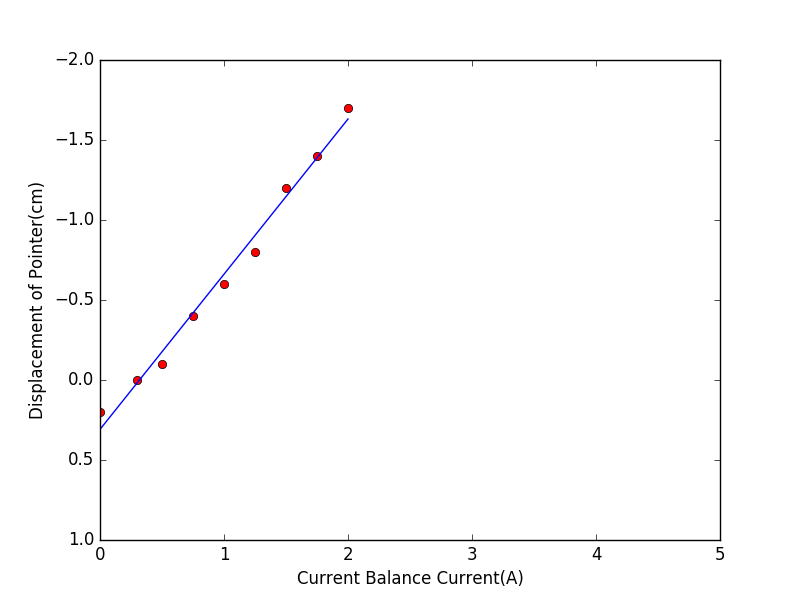
\includegraphics[width=0.45\textwidth]{img/figure_1.png}
			}
			\subfigure[파란색:+0.1\si{cm}, 초록색:-0.1\si{cm}의 오차가 허용된 추세선]{
				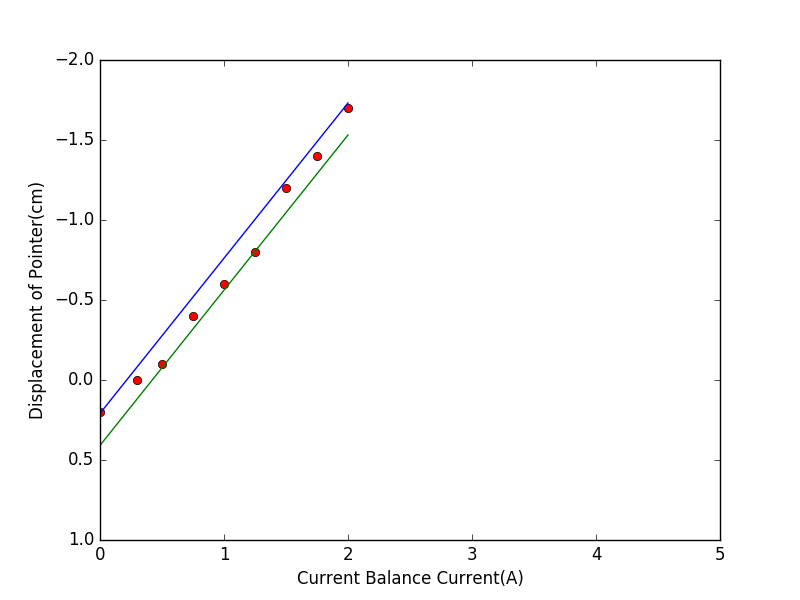
\includegraphics[width=0.45\textwidth]{img/figure_1-error.png}
				\label{fig:error1}
			}
		\end{figure}
		천칭에 인가된 전류를 바꾸어가며 그에 따른 가리키게의 길이와 변위의 변화를 표와 그래프로 나타낸 것이다.
		측정장비의 오차를 반영하여 가리키게의 변위에 $\mypm{}0.1\si{cm}$의 오차를 반영한 그래프도 그렸다. 

		\subsection{솔레노이드의 전류에 따른 토크의 변화}

		\begin{figure}[h]
			\centering
				\begin{tabular}{cccccc} 
					\hline \hline
					전류(A) \qquad \qquad \vline & 0.5 & 1.0 & 1.5 & 2.0 & 2.5 \\
					\hline
					가리키게 눈금(\si{cm}) \vline & 9.9 & 9.9 & 9.9 & 10.0 & 10.5 \\
					\hline
					가리키게 변위(\si{cm}) \vline & -0.5 & -0.9 & -1.3 & -1.8 & -2.4 \\
					\hline \hline
				\end{tabular}  
			\label{tb:soloutput}
		\end{figure}

		\vspace{-0.5cm}
		
		\begin{figure}[h]
			\centering
			\subfigure[솔레노이드에 인가된 전류와 그에 따른 가리키게의 위치변화]{
				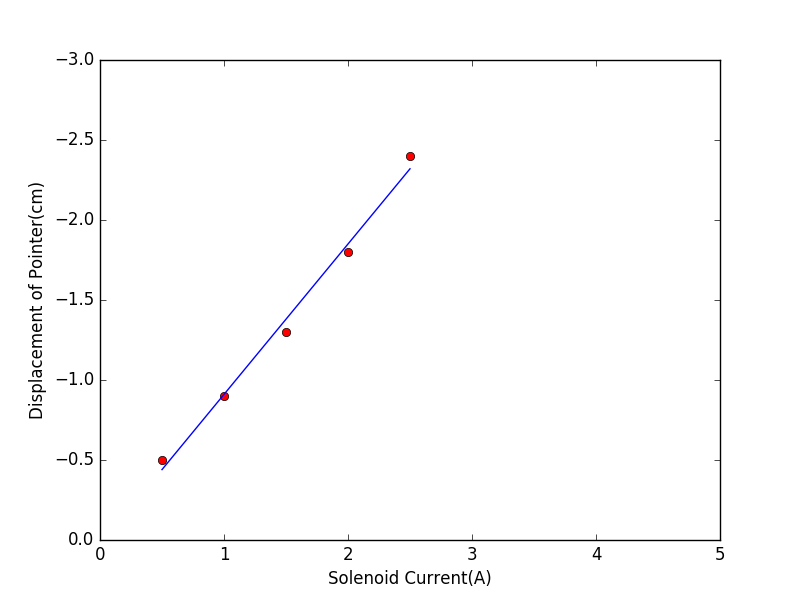
\includegraphics[width=0.45\textwidth]{img/figure_2.png}
			}
			\subfigure[파란색:+0.1\si{cm}, 초록색:-0.1\si{cm}의 오차가 허용된 추세선]{
				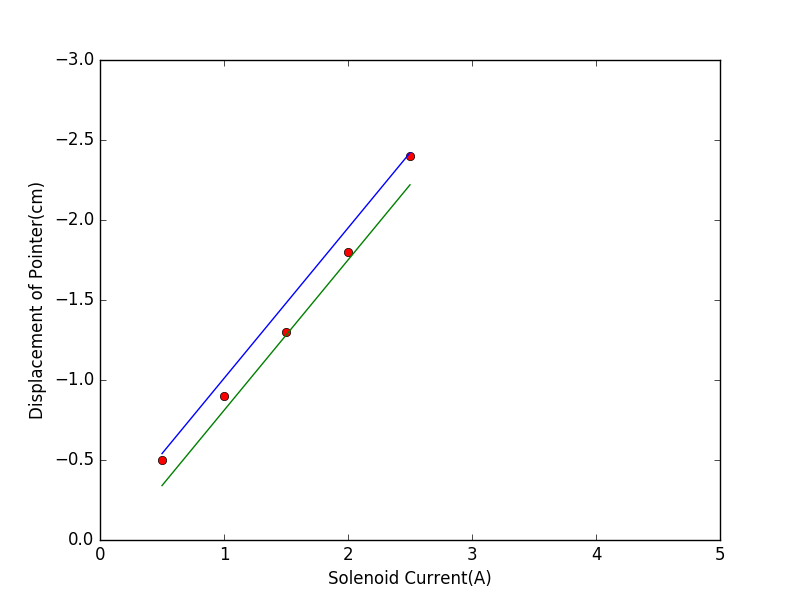
\includegraphics[width=0.45\textwidth]{img/figure_2-error.png}
				\label{fig:error2}
			}
		\end{figure}
		솔레노이드에 인가된 전류를 바꾸어가며 그에 따른 가리키게의 길이와 변위의 변화를 표와 그래프로 나타낸 것이다.
		측정장비의 오차를 반영하여 가리키게의 변위에 $\mypm{}0.1\si{cm}$의 오차를 반영한 그래프도 그렸다.

	

\newpage




	\section{Conclusion}
	식(1.8)과 식(1.9)은 전류가 증가함에 따라 전류천칭의 변위값이 선형적으로 증가할 것으로 예측했고 Scipy로 Line Regression을 해본 결과 두 실험 모두 R값이 0.9884, 0.9915로 매우 직선에 가까운 것으로 나타났다.
	따라서 Introduction에서 유도했던 식들과 그 기본이 되는 앙페르 법칙과 로렌츠 힘은 참이라고 볼 수 있다. 

	솔레노이드의 규격, 천칭의 규격등은 모두 실험실에서 측정되었으나 천칭의 무게중심과 받침점 사이의 거리인 $d$를 측정하지 못했기 때문에 실험과 이론의 비례상수를 비교하지는 못했다. 

	오차분석을 해보면 첫 번째로 $\Delta{}x$가 $F$와 선형적으로 비례하지 않는 것을 원인으로 들 수 있다. 
	실제로는 $\sin{\Delta{}x}$에 비례하는 값이어야 한다.
	그럼에도 실험값이 직선형에 가깝게 나온 것은 가리키게의 변위(최대 2.4\si{cm})보다 천칭의 길이(24\si{cm})가 훨씬 커서 $\theta$가 매우 작기 때문으로 보인다.
	$\theta=\frac{2.4}{24}=0.1$에서 $y=x$와 $y=sinx$의 상대오차는 $\frac{0.1-\sin{0.1}}{0.1}=1.6 \times 10^{-3}$으로 우리의 측정장비(0.2\si{cm})의 한계로 측정되지 않는 수준이다. 
	두 번째는 천칭 받침점의 마찰력으로 생각된다.
	실험을 할 때 전류를 바꿨음에도 천칭이 기울어진 각도가 변하지 않는 경우가 있었다.
	이런 경우, 천칭을 손으로 살짜 건드려준 후에야 새로운 평형 각도로 옮겨가는 것을 볼 수 있었다.
	이러한 결과는 유의미한 마찰력의 존재를 시사한다.
	
	그러나 실험이 전반적으로 이론적인 예측과 잘 일치했고 두 실험의 그래프에 나타나듯이 오차에 방향성이 없는 것을 보아 오차의 대부분은 우연오차로 보는 것이 타당하다.
		
	그러나 이러한 오차들은 실험기구의 정밀성을 고려하면 모두 허용될 수 있는 범위의 오차다.
	가리키게의 눈금은 0.2\si{cm}였는데 눈으로 이 값을 측정할 때 두 눈금 사이에 값이 위치하는 경우가 많았다.
	그래서 실험자는 두 눈금 사이에 가리키게가 위치했을 때 임의적으로 0.1\si{cm}로 끊었다.
	이를 반영하여 Result의 그래프(\ref{fig:error1})에서 $\mypm{}0.1\si{cm}$의 오차를 허용하면 모든 점들이 두 직선 사이에 들어가는 것을 볼 수 있었다.
	이로부터 결과의 오차는 측정 장비의 정밀도에 많은 영향을 받았음을 알 수 있었다.




\section{Reference 및 부록}
	1. Halliday, D., Resnick, R., \& Walker, J. (2014). {\it{}Principles of Physics} (10th ed., Vol. 2). Hoboken, NJ: Wiley.
	\\ 

\end{document} 

%실험에서 개선할 점 등 피피티에서 봤던 거 모두 적어서 처리합시다